\documentclass[12pt,a4paper]{article}
\usepackage[utf8]{inputenc}
\usepackage{dsfont} 
\usepackage[brazilian]{babel}
\usepackage{amsmath}
\usepackage{graphicx}
\usepackage[top=1in, bottom=1.5in, left=1.25in, right=1.25in]{geometry}

\usepackage{subfig}
\usepackage{multirow}
\usepackage{multicol}
\graphicspath{{imagens/}}
\usepackage{xcolor,colortbl}
\usepackage{float}

\newcommand \comment[1]{\textbf{\textcolor{red}{#1}}}

%\usepackage{float}
\usepackage{fancyhdr} % Required for custom headers
\usepackage{lastpage} % Required to determine the last page for the footer
\usepackage{extramarks} % Required for headers and footers
\usepackage{indentfirst}
\usepackage{placeins}
\usepackage{scalefnt}

% Margins
\addtolength{\footskip}{0cm}
\addtolength{\textwidth}{1.4cm}
\addtolength{\oddsidemargin}{-.7cm}

\addtolength{\textheight}{1.6cm}
%\addtolength{\topmargin}{-2cm}

% paragrafo
\addtolength{\parskip}{.2cm}

% Set up the header and footer
\pagestyle{fancy}
%\rhead{\hmwkAuthorName} % Top left header
%\lhead{\hmwkClass: \hmwkTitle} % Top center header
%\rhead{\firstxmark} % Top right header
\lfoot{Lucas Santos, Matheus Barbosa, Rafael Sidnei.} % Bottom left footer
\cfoot{} % Bottom center footer
\rfoot{} % Bottom right footer
\renewcommand{\headrulewidth}{1pt}
\renewcommand{\footrulewidth}{1pt}
%----------------------------------------------------------------------------------------
%	Nome e Disciplina
%----------------------------------------------------------------------------------------
    
\newcommand{\hmwkTitle}{Trabalho Final} % Assignment title
\newcommand{\hmwkDueDate}{Dezembro de 2018} % Due date
\newcommand{\hmwkClass}{Banco de Dados} % Course/class
\newcommand{\hmwkAuthorName}{Lucas Nogueira Santos, Matheus Barbosa Souza, Rafael Sidnei Alves} % Your name

% trabalho 
\begin{document}
% capa
\begin{titlepage}
    \vfill
	\begin{center}
    
\includegraphics[scale=1.0]{imagens/logo.png}\\
	\textbf{UNIVERSIDADE PRESIDENTE ANTÔNIO CARLOS \\ CIÊNCIA DA COMPUTAÇÃO}

	\vspace{0.6cm}
	\vspace{4cm}
	{\huge \textbf{Trabalho Final}}
	
	{\huge \textbf{Análise de Bases}}\vspace{8mm}
	
	{\large \textbf{Lucas Nogueira Santos \\ Matheus Barbosa Souza \\ Rafael Sidnei Alves}}\\[3cm]
	
		\hspace{.45\textwidth} %posiciona a minipage
	   \begin{minipage}{.5\textwidth}
	   Trabalho teórico apresentado à disciplina de Inteligência Artificial do curso de Ciência da Computação da Universidade Presidente Antônio Carlos.\\[0.1cm]
	  \end{minipage}
	  \vfill
	%\vspace{2cm}
	
	\textbf{Barbacena}
	
	\textbf{Dezembro de 2018}
	\end{center}
	
\end{titlepage}

% Sumario
\newpage
\setcounter{secnumdepth}{5}
\tableofcontents
\newpage

\section{Introdução}
\label{sec:introducao}

A história da computação é marcada por períodos de inovação disruptiva que muda completamente o cenário da tecnologia.E os gerenciadores de banco de dados pareciam imunes a mudanças de paradigma. Mas desde 2004, o cenário começou a mudar e agora a mudança parece inevitável. A prova disso, é que os grandes players do mercado, Oracle, IBM e Microsoft, estão revendo seus produtos, que juntos representam mais de 90\% do mercado de bancos de dados.

Para empresas que estão selecionando produtos de banco de dados para um tipo específico de aplicativo, nosso conselho é determinar qual categoria de banco de dados eles precisam antes de pensar em quais produtos investigar. Embora, com o passar do tempo, possamos esperar que haja alguma racionalização entre essas categorias de bancos de dados, esperamos que a maioria deles persista com dois ou três produtos dominando cada categoria. Isso ocorre porque as categorias foram derivadas com base em diferentes tipos de carga de trabalho, e não esperamos que um mecanismo de banco de dados que seja excelente em uma dessas categorias tenha um desempenho particularmente bom em outras categorias.

Sistemas Gerenciadores de Bancos de dados são usados em muitas aplicações, enquanto atravessando virtualmente a gama inteira de software de computador. Os Sistemas Gerenciadores de Bancos de dados são o método preferido de armazenamento/recuperação de dados/informações para aplicações multiusuárias grandes onde a coordenação entre muitos usuários é necessária. Até mesmo usuários individuais os acham conveniente, entretanto, muitos programas de correio eletrônico e organizadores pessoais estão baseados em tecnologia de banco de dados standard. \newpage
\section{Redes Neurais}
\label{sec:redesneurais}

A primeira inteligência utilizada foi a Redes Neurais.

Como pode-se observar a melhor base a ser utilizada em Redes Neurais é a Car, tendo acurácia de 95,73\%, em seguida vem a base Adult e a WPBC com 77,95\% e 77,23\% respectivamente, por último, as bases com menor acurácia foram Abalone e Yeast com 55,68\% e 44,21\% respectivamente. Uma curiosidade é que as bases Adult e WPBC tiveram um desempenho relativamente próximo.

O gráfico abaixo mostra com clareza os resultados de todas as bases com seus valores máximos e mínimos, e claro, sua média para definir qual a melhor.

\begin{center}
      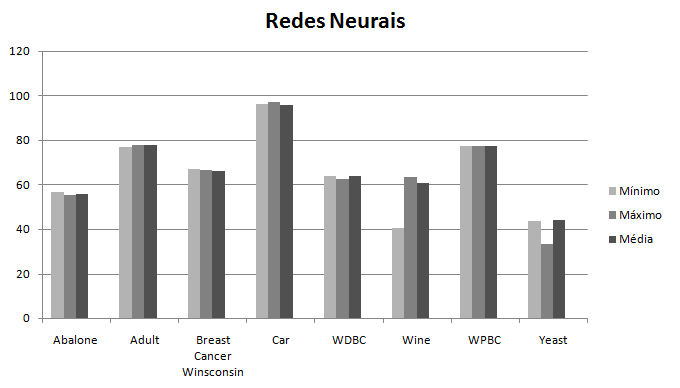
\includegraphics[scale=1.0]{imagens/redesneurais.png}
\end{center}
 
 \newpage
\section{Árvore de Decisão}
\label{sec:arvore}

A segunda inteligência utilizada foi a Árvore de Decisão.

Como pode-se observar a melhor base a ser utilizada na Árvore de Decisão é a Breast Cancer Winsconsin, tendo acurácia de 89,46\%, em seguida vem a base Car e a Adult com 86,16\% e 84,51\% respectivamente, por último, as bases com menor acurácia foram Abalone e Yeast com 53,15\% e 51,21\% respectivamente.

O gráfico abaixo mostra com clareza os resultados de todas as bases com seus valores máximos e mínimos, e claro, sua média para definir qual a melhor.

\begin{center}
      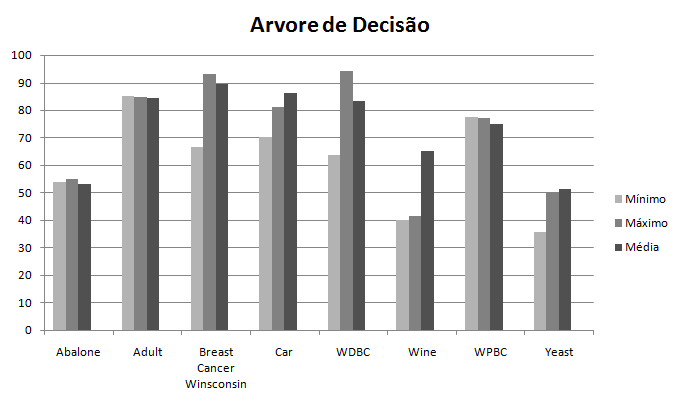
\includegraphics[scale=1.0]{imagens/arvore.png}
\end{center} \newpage
\section{SVM Learner}
\label{sec:arvore}

A penúltima inteligência utilizada foi a SVM Learner.

Como pode-se observar a melhor base a ser utilizada na SVM é a Car, tendo acurácia de 80,76\%, em seguida vem a base Adult com 79,52\% (as demais bases tiveram valores relativamente baixos), por último, as bases com menor acurácia foram WDBC e Yeast com 57,94\% e 41,74\% respectivamente.

O gráfico abaixo mostra com clareza os resultados de todas as bases com seus valores máximos e mínimos, e claro, sua média para definir qual a melhor.

\begin{center}
      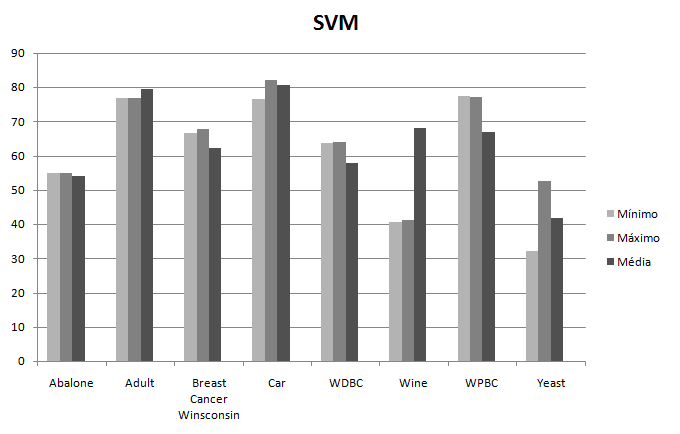
\includegraphics[scale=1.0]{imagens/svm.png}
\end{center} \newpage
\section{KNN}
\label{sec:arvore}

A última inteligência utilizada foi a KNN Learner.

Como pode-se observar a melhor base a ser utilizada na KNN é a Car, tendo acurácia de 93,88\%, em seguida vem a base Adulte a WDBC com 76,96\% e 74,15\% respectivamente, por último, as bases com menor acurácia foram Breast Cancer Winsconsin e Yeast com 66,05\% e 50,02\% respectivamente.

O gráfico abaixo mostra com clareza os resultados de todas as bases com seus valores máximos e mínimos, e claro, sua média para definir qual a melhor.

\begin{center}
      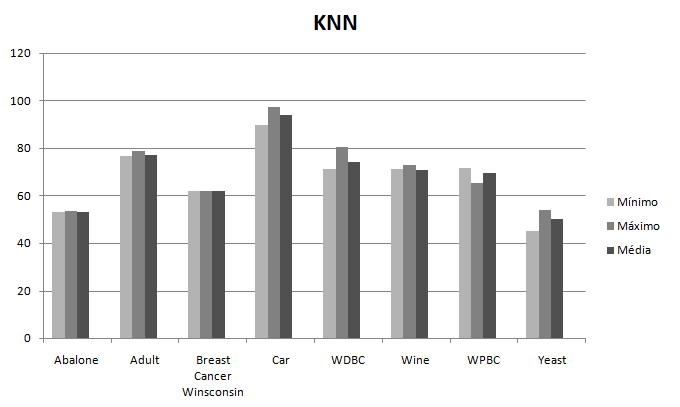
\includegraphics[scale=1.0]{imagens/knn.png}
\end{center} \newpage
\section{Resultados}
\label{sec:introducao}

Com base nos testes realizados em relação aos resultados das médias de cada inteligência podemos ver que a base Car teve maior acurácia em todas as inteligências exceto pela SVM Learner, o que a torna a melhor base em estudo.

\begin{center}
      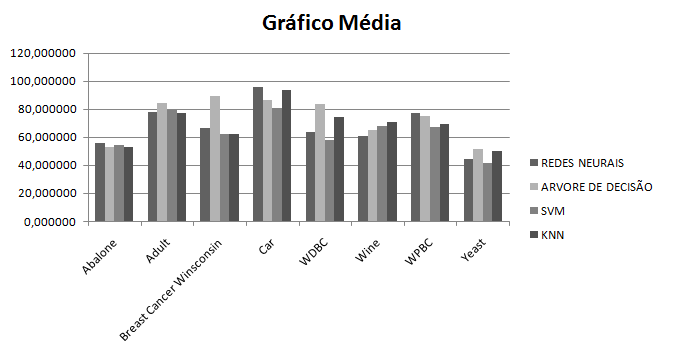
\includegraphics[scale=1.0]{imagens/media.png}
\end{center}

Após a interpretação do gráfico definimos cada base com sua melhor e pior inteligência:

\begin{itemize}
    \item \textbf{Abalone}: A melhor inteligência a ser usada nessa base é a Redes Neurais com 55,68\% enquanto a pior é a KNN com 53,00\%;
    \item \textbf{Adult}: A melhor inteligência a ser usada nessa base é a Árvore de Decisão com 84,51\% enquanto a pior é a KNN com 76,96\%;
    \item \textbf{Breast Cancer Winsconsin}: A melhor inteligência a ser usada nessa base é a Árvore de Decisao com 89,46\% enquanto a pior é a KNN com 62,05\%;
    \item \textbf{Car}: A melhor inteligência a ser usada nessa base é a Redes Neurais com 95,73\% enquanto a pior é a SVM com 80,76\%;
    \item \textbf{WDBC}: A melhor inteligência a ser usada nessa base é a Árvore de Decisão com 83,27\% enquanto a pior é a SVM com 57,94\%;
    \item \textbf{Wine}: A melhor inteligência a ser usada nessa base é a KNN com 70,69\% enquanto a pior é a Redes Neurais com 60,60\%;
    \item \textbf{WPBC}: A melhor inteligência a ser usada nessa base é a Redes Neurais com 77,23\% enquanto a pior é a SVM com 69,51\%;
    \item \textbf{Abalone}: A melhor inteligência a ser usada nessa base é a Árvore de Decisão com 51,21\% enquanto a pior é a SVM com 41,74\%.
\end{itemize}

\end{document}